\documentclass[conference]{IEEEtran}
\usepackage{graphicx}
\usepackage{amsmath}
\usepackage{booktabs}
\usepackage{url}
\usepackage{array}
\usepackage{tikz}
\usetikzlibrary{arrows.meta,positioning,calc}
\usepackage{pgfplots}
\pgfplotsset{compat=1.17}

\begin{document}

\title{Design and Analysis of a Direct-Mapped\\Cache Controller in Verilog}

\author{
\IEEEauthorblockN{Asad Ali, Divyansh Bhartia, Vikrant Yadav, Mayank Pillai, Prashant Raj}
\IEEEauthorblockA{Project 6 --- Modern Computer Architecture}
}

\maketitle

\begin{abstract}
A cache is a small, fast memory that keeps recently used data close to the processor so that most memory
accesses do not have to wait for the slow main memory. We design, simulate and synthesise a 1~KB
direct-mapped cache with 16-byte blocks and 32-bit addresses in Verilog. The design is split into the modules
suggested for the project: an address decoder, valid-bit, tag and data RAMs, a tag comparator, a four-state
controller finite-state machine (FSM) and a main-memory interface. Reads use a refill-on-miss policy and writes use
write-through with no-write-allocate. A self-checking testbench replays memory-access traces (sequential, repeated,
random, conflict and mixed read/write), compares every value read with a reference memory and reports hit ratio,
miss ratio and average memory access time (AMAT). With a 10-cycle main memory the hit time is 2 cycles and the
miss penalty 12 cycles. The sequential trace reaches a 75\% hit ratio (AMAT 5.0 cycles), the repeated loop 97.5\%
(2.3 cycles), random accesses 1.1\% (13.9 cycles) and the conflict trace 0\% (14.0 cycles). The AMAT measured in
simulation equals the formula value in every case and no data errors were found. Yosys synthesis for a Xilinx
7-series FPGA uses 316 LUTs, 138 flip-flops and 136 distributed-RAM primitives.
\end{abstract}

\begin{IEEEkeywords}
cache memory, direct-mapped cache, cache controller, finite-state machine, AMAT, Verilog, locality
\end{IEEEkeywords}

% ======================================================================
\section{Introduction}
Processors run much faster than main memory (DRAM). If every load and store waited for DRAM, the processor would
spend most of its time idle. Caches solve this by keeping a copy of recently used data in a small, fast memory next
to the processor~\cite{hennessy2017}. Caches work because programs show \emph{locality}~\cite{denning2005}:
\begin{itemize}
\item \textbf{Temporal locality} --- data used now is likely to be used again soon (e.g.\ loop variables).
\item \textbf{Spatial locality} --- data near a used address is likely to be used soon (e.g.\ array elements).
\end{itemize}
The simplest cache organisation is the \emph{direct-mapped} cache, in which every memory block can be stored in
exactly one cache line. This makes the lookup a single tag comparison, so the hardware is small and fast.

The goal of this project is to design a direct-mapped cache controller in Verilog and to analyse its hit/miss
behaviour on representative memory-access traces. Our contributions are:
\begin{itemize}
\item a modular, synthesisable Verilog cache (1~KB, 16-byte blocks, 32-bit addresses) with a 4-state controller;
\item a self-checking testbench and six memory-access traces that show the effect of locality and conflicts;
\item hit ratio, miss ratio and AMAT measurements, a memory-latency sweep and FPGA synthesis results.
\end{itemize}

% ======================================================================
\section{Literature Review}
\textbf{Cache fundamentals.} Smith's survey~\cite{smith1982} describes the main design choices of a cache:
placement (direct-mapped, set-associative, fully associative), block size, replacement and write policy. Hennessy
and Patterson~\cite{hennessy2017} define the average memory access time,
\begin{equation}
\text{AMAT} = \text{Hit time} + \text{Miss rate} \times \text{Miss penalty},
\label{eq:amat}
\end{equation}
which we use as the main performance metric. They also classify misses into the ``three Cs'':
\emph{compulsory} (first access to a block), \emph{capacity} (the working set does not fit) and
\emph{conflict} (two blocks compete for the same line).

\textbf{Direct-mapped versus associative caches.} Hill~\cite{hill1988} argued that direct-mapped caches can
outperform set-associative ones in practice, because their shorter hit time can outweigh their higher miss ratio.
Hill and Smith~\cite{hill1989} measured how associativity changes miss ratios and found that moving from direct-mapped
to two-way removes a large part of the conflict misses. Jouppi~\cite{jouppi1990} kept the fast direct-mapped cache
and removed many conflict misses by adding a small fully associative \emph{victim cache}.

\textbf{Cache controller design.} Patterson and Hennessy~\cite{patterson2020} present a simple cache controller as a
four-state FSM (Idle, Compare Tag, Write-Back, Allocate) for a write-back cache. We follow the same structure, but
replace the write-back state with a write-to-memory state because we use a write-through policy, which needs no
dirty bits and is easier to verify.

\textbf{Tools.} The design is written in Verilog (IEEE~1364~\cite{ieee1364}), simulated with Icarus
Verilog~\cite{iverilog} and synthesised with Yosys~\cite{yosys}, which are free, open-source tools.

% ======================================================================
\section{Proposed Solution}

\subsection{Cache parameters and address fields}
The cache stores 1024 bytes in blocks of 16 bytes, so it has $1024/16 = 64$ lines. A 32-bit byte address is split
into three fields (Table~\ref{tab:addr}):
\begin{itemize}
\item \textbf{Offset} (4 bits): $\log_2 16 = 4$; bits [3:2] choose one of the 4 words in a block.
\item \textbf{Index} (6 bits): $\log_2 64 = 6$; chooses the cache line.
\item \textbf{Tag} (22 bits): the remaining $32-6-4$ bits; identifies which memory block is in the line.
\end{itemize}

\begin{table}[h]
\centering
\caption{Address breakdown (32-bit address)}
\label{tab:addr}
\begin{tabular}{lccc}
\toprule
Field & Tag & Index & Offset \\
\midrule
Bits  & 31--10 & 9--4 & 3--0 \\
Width & 22 & 6 & 4 \\
Example \texttt{0x0000\_0404} & \texttt{0x000001} & 0 & 4 (word 1) \\
\bottomrule
\end{tabular}
\end{table}

The total storage is $64 \times (128 + 22 + 1) = 9664$ bits, of which 8192 are data. Addresses that differ by a
multiple of 1~KB have the same index and therefore \emph{conflict} for the same line.

\subsection{Architecture}
Fig.~\ref{fig:block} shows the block diagram. Each box is one Verilog module:
\begin{itemize}
\item \texttt{address\_decoder} --- splits the latched address into tag, index and word select (wiring only).
\item \texttt{valid\_ram} --- 64 valid bits, all cleared on reset, so the cache starts empty.
\item \texttt{tag\_ram} --- 64 tags of 22 bits.
\item \texttt{data\_ram} --- 64 blocks of 128 bits; can write a whole block (refill) or one word (store hit).
\item \texttt{tag\_comparator} --- $\text{hit} = \text{valid} \wedge (\text{stored tag} = \text{address tag})$.
\item \texttt{cache\_controller} --- the FSM that sequences lookup, refill and memory writes.
\item \texttt{main\_memory} --- a 64~KB memory model with a configurable latency $L$ (10 cycles by default),
      that returns a whole 16-byte block on a read.
\item \texttt{cache\_top} --- connects the modules and holds the request registers.
\end{itemize}
All RAMs are read asynchronously, so the tag check and data read finish in one clock cycle.

\begin{figure}[t]
\centering
\resizebox{\columnwidth}{!}{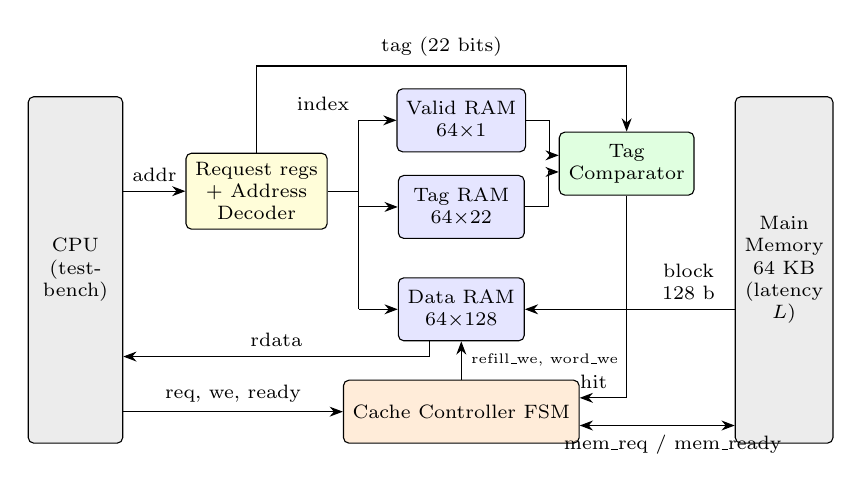
\begin{tikzpicture}[font=\scriptsize, >=Stealth,
  blk/.style={draw, rounded corners=2pt, align=center, minimum height=0.8cm, fill=#1},
  blk/.default=white]
  % columns: CPU | decoder | RAMs | comparator | memory
  \node[blk=gray!15, minimum width=1.2cm, minimum height=4.4cm] (cpu) at (0,0) {CPU\\(test-\\bench)};
  \node[blk=yellow!15, minimum width=1.6cm] (dec) at (2.3,1.0) {Request regs\\+ Address\\Decoder};
  \node[blk=blue!10, minimum width=1.6cm] (valid) at (4.9,1.9) {Valid RAM\\64$\times$1};
  \node[blk=blue!10, minimum width=1.6cm] (tag)   at (4.9,0.8) {Tag RAM\\64$\times$22};
  \node[blk=blue!10, minimum width=1.6cm] (data)  at (4.9,-0.5) {Data RAM\\64$\times$128};
  \node[blk=green!12, minimum width=1.3cm] (cmp)  at (7.0,1.35) {Tag\\Comparator};
  \node[blk=orange!15, minimum width=2.6cm] (fsm) at (4.9,-1.8) {Cache Controller FSM};
  \node[blk=gray!15, minimum width=1.2cm, minimum height=4.4cm] (mem) at (9.0,0) {Main\\Memory\\64 KB\\(latency\\$L$)};

  % address path
  \draw[->] (cpu.east |- dec.west) -- node[above]{addr} (dec.west);
  \coordinate (bus) at (3.6,0);
  \draw (dec.east) -- (dec.east -| bus);
  \draw (bus |- valid.west) -- (bus |- data.west);
  \draw[->] (bus |- valid.west) -- (valid.west);
  \draw[->] (bus |- tag.west) -- (tag.west);
  \draw[->] (bus |- data.west) -- (data.west);
  \node[above left] at (bus |- valid.west) {index};
  \draw[->] (dec.north) -- ++(0,1.1) -| node[pos=0.25,above]{tag (22 bits)} (cmp.north);
  % comparator inputs / output
  \draw[->] (valid.east) -- ++(0.3,0) |- ([yshift=3pt]cmp.west);
  \draw[->] (tag.east) -- ++(0.3,0) |- ([yshift=-3pt]cmp.west);
  \draw[->] (cmp.south) |- node[pos=0.85,above]{hit} ([yshift=5pt]fsm.east);
  % data out
  \draw[->] ([xshift=4mm]data.south west) |- node[pos=0.75,above]{rdata} (cpu.east |- 0,-1.1);
  % control
  \draw[->] (cpu.east |- fsm.west) -- node[above]{req, we, ready} (fsm.west);
  \draw[<->] ([yshift=-5pt]fsm.east) -- node[below, pos=0.6]{mem\_req / mem\_ready} ([yshift=-5pt]fsm.east -| mem.west);
  \draw[->] (mem.west |- data.east) -- node[above, pos=0.22, align=center]{block\\128 b} (data.east);
  \draw[->] (fsm.north) -- node[right]{\tiny refill\_we, word\_we} (data.south);
\end{tikzpicture}
}
\caption{Block diagram of the direct-mapped cache.}
\label{fig:block}
\end{figure}

\subsection{Controller FSM}
The controller (Fig.~\ref{fig:fsm}) has four states:
\begin{enumerate}
\item \textbf{IDLE}: wait for \texttt{cpu\_req}; latch the address, write data and read/write flag.
\item \textbf{COMPARE}: check the valid bit and the tag. On a \emph{read hit} the word is returned and
\texttt{cpu\_ready} is raised. On a \emph{read miss} the FSM goes to ALLOCATE. On a \emph{write}, the word is
updated in the cache if it hits and the FSM goes to WRITE\_MEM.
\item \textbf{ALLOCATE}: request the block from main memory. When \texttt{mem\_ready} arrives, the block, tag and
valid bit are written in one cycle and the FSM returns to COMPARE, which now hits.
\item \textbf{WRITE\_MEM}: write the word to main memory (write-through), then raise \texttt{cpu\_ready}.
\end{enumerate}
Write misses do not load the block into the cache (\emph{no-write-allocate}). The controller also outputs one-cycle
\texttt{stat\_hit}/\texttt{stat\_miss} pulses on the first comparison of each request, which the testbench counts.

\begin{figure}[t]
\centering
\resizebox{0.95\columnwidth}{!}{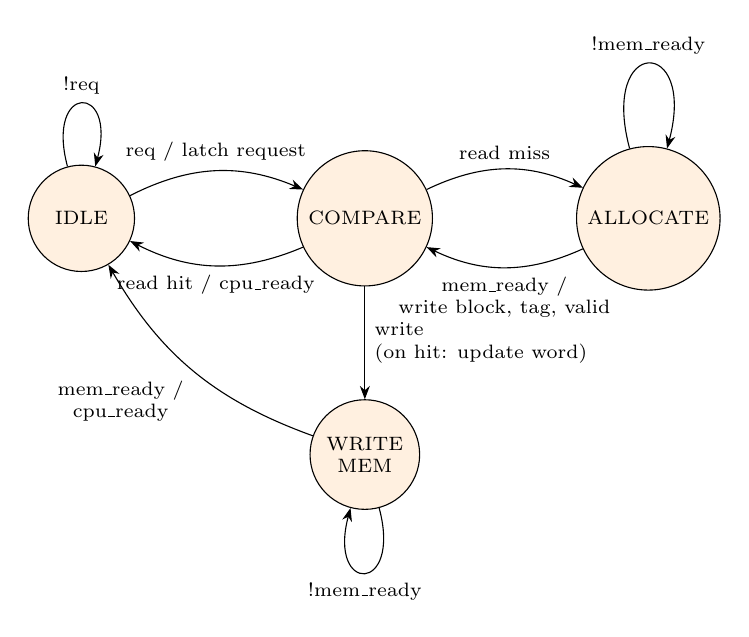
\begin{tikzpicture}[font=\scriptsize, >=Stealth,
  st/.style={draw, circle, minimum size=1.35cm, align=center, fill=orange!12}]
  \node[st] (idle)  at (0,0)    {IDLE};
  \node[st] (cmp)   at (3.6,0)  {COMPARE};
  \node[st] (alloc) at (7.2,0)  {ALLOCATE};
  \node[st] (wmem)  at (3.6,-3) {WRITE\\MEM};

  \draw[->] (idle) to[loop above] node{!req} (idle);
  \draw[->] (idle) to[bend left=25] node[above]{req / latch request} (cmp);
  \draw[->] (cmp) to[bend left=25] node[below]{read hit / cpu\_ready} (idle);

  \draw[->] (cmp) to[bend left=25] node[above]{read miss} (alloc);
  \draw[->] (alloc) to[bend left=25] node[below, align=center]{mem\_ready /\\write block, tag, valid} (cmp);
  \draw[->] (alloc) to[loop above] node{!mem\_ready} (alloc);

  \draw[->] (cmp) -- node[right, align=left]{write\\(on hit: update word)} (wmem);
  \draw[->] (wmem) to[bend left=20] node[below left, align=center]{mem\_ready /\\cpu\_ready} (idle);
  \draw[->] (wmem) to[loop below] node{!mem\_ready} (wmem);
\end{tikzpicture}
}
\caption{Cache controller FSM.}
\label{fig:fsm}
\end{figure}

\subsection{Timing}
A hit takes 2 cycles (IDLE $\rightarrow$ COMPARE $\rightarrow$ IDLE). A read miss takes
$2 + (L + 2) = 14$ cycles for $L = 10$: IDLE and COMPARE as for a hit, then $L + 1$ cycles in ALLOCATE ($L$ cycles
of memory latency plus the cycle in which the block is written), and a second COMPARE that now hits. Hence the \textbf{hit time is 2 cycles and the miss penalty is
$L + 2 = 12$ cycles}, so by~\eqref{eq:amat}
\begin{equation}
\text{AMAT} = 2 + \text{Miss rate} \times 12 \ \text{cycles}.
\end{equation}

\subsection{Verification method and traces}
The testbench (\texttt{tb\_cache.v}) reads a trace file in which each line is \texttt{R addr} or
\texttt{W addr data}. Main memory is initialised so that the word at address $A$ holds the value $A$, which makes
results easy to check by eye. The testbench keeps its own reference memory, checks every value read, counts hits,
misses and cycles, and writes a per-access log and a CSV summary. A Python script generates six traces:
\begin{itemize}
\item \textbf{sequential}: read 4~KB word by word (spatial locality);
\item \textbf{repeated}: read a 512-byte array 10 times (temporal locality);
\item \textbf{random}: 1000 random words in 64~KB (little locality);
\item \textbf{conflict}: alternate between \texttt{0x040} and \texttt{0x440}, which share line 4;
\item \textbf{mixed}: 200 reads and writes (30\% writes) in 2~KB, to test write-through;
\item \textbf{demo}: 8 hand-picked accesses that show a cold miss, hits, a conflict miss and a write hit.
\end{itemize}

% ======================================================================
\section{Results and Discussion}

\subsection{Functional verification}
All six traces finish with zero data errors, so every read returned the correct value, including reads after
writes. Fig.~\ref{fig:wave} shows the start of the demo trace: the first read of \texttt{0x000} misses (cold
miss, valid bit 0), the FSM spends 10 cycles in ALLOCATE waiting for memory, and the next reads of \texttt{0x004}
and \texttt{0x00C} hit in 2 cycles because they are in the block that was just loaded. Later in the trace,
\texttt{0x400} replaces block \texttt{0x000} in line 0 (same index, different tag), so the following read of
\texttt{0x000} misses again.

\begin{figure*}[t]
\centering
\resizebox{0.9\textwidth}{!}{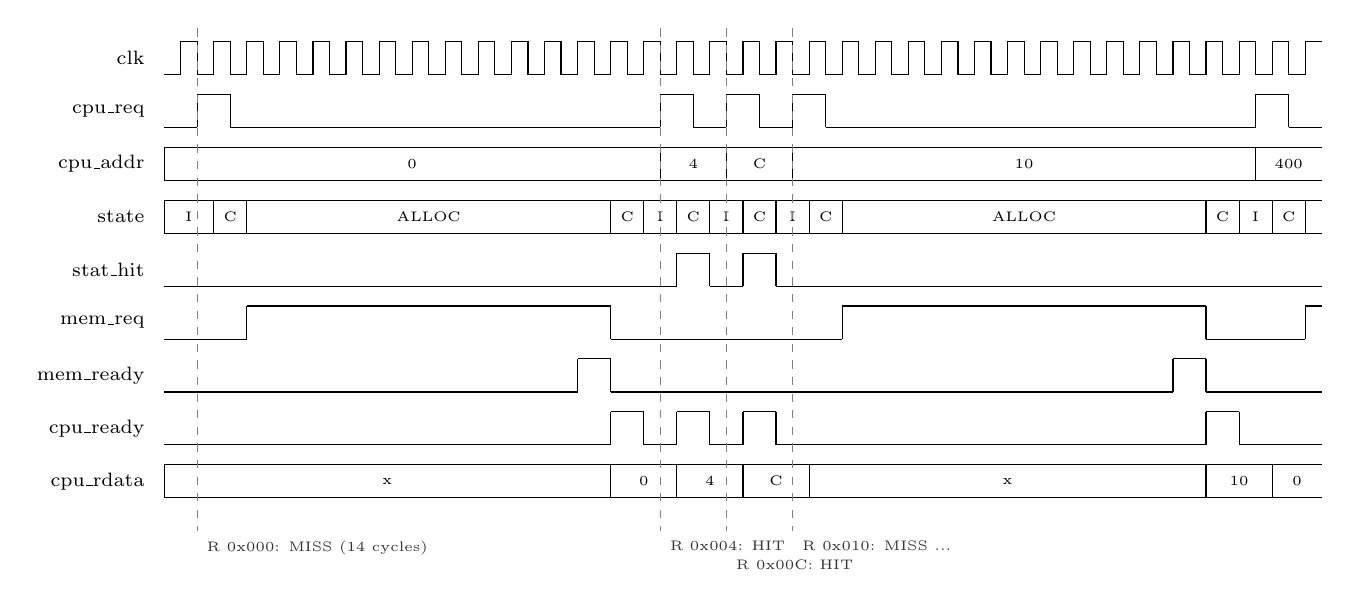
\begin{tikzpicture}[x=0.042cm,y=0.42cm,font=\scriptsize]
\node[anchor=east] at (27,0.50) {clk};
\draw (30,0.00) -- (35,0.00);
\draw (35,0.00) -- (35,1.00);
\draw (35,1.00) -- (40,1.00);
\draw (40,0.00) -- (40,1.00);
\draw (40,0.00) -- (45,0.00);
\draw (45,0.00) -- (45,1.00);
\draw (45,1.00) -- (50,1.00);
\draw (50,0.00) -- (50,1.00);
\draw (50,0.00) -- (55,0.00);
\draw (55,0.00) -- (55,1.00);
\draw (55,1.00) -- (60,1.00);
\draw (60,0.00) -- (60,1.00);
\draw (60,0.00) -- (65,0.00);
\draw (65,0.00) -- (65,1.00);
\draw (65,1.00) -- (70,1.00);
\draw (70,0.00) -- (70,1.00);
\draw (70,0.00) -- (75,0.00);
\draw (75,0.00) -- (75,1.00);
\draw (75,1.00) -- (80,1.00);
\draw (80,0.00) -- (80,1.00);
\draw (80,0.00) -- (85,0.00);
\draw (85,0.00) -- (85,1.00);
\draw (85,1.00) -- (90,1.00);
\draw (90,0.00) -- (90,1.00);
\draw (90,0.00) -- (95,0.00);
\draw (95,0.00) -- (95,1.00);
\draw (95,1.00) -- (100,1.00);
\draw (100,0.00) -- (100,1.00);
\draw (100,0.00) -- (105,0.00);
\draw (105,0.00) -- (105,1.00);
\draw (105,1.00) -- (110,1.00);
\draw (110,0.00) -- (110,1.00);
\draw (110,0.00) -- (115,0.00);
\draw (115,0.00) -- (115,1.00);
\draw (115,1.00) -- (120,1.00);
\draw (120,0.00) -- (120,1.00);
\draw (120,0.00) -- (125,0.00);
\draw (125,0.00) -- (125,1.00);
\draw (125,1.00) -- (130,1.00);
\draw (130,0.00) -- (130,1.00);
\draw (130,0.00) -- (135,0.00);
\draw (135,0.00) -- (135,1.00);
\draw (135,1.00) -- (140,1.00);
\draw (140,0.00) -- (140,1.00);
\draw (140,0.00) -- (145,0.00);
\draw (145,0.00) -- (145,1.00);
\draw (145,1.00) -- (150,1.00);
\draw (150,0.00) -- (150,1.00);
\draw (150,0.00) -- (155,0.00);
\draw (155,0.00) -- (155,1.00);
\draw (155,1.00) -- (160,1.00);
\draw (160,0.00) -- (160,1.00);
\draw (160,0.00) -- (165,0.00);
\draw (165,0.00) -- (165,1.00);
\draw (165,1.00) -- (170,1.00);
\draw (170,0.00) -- (170,1.00);
\draw (170,0.00) -- (175,0.00);
\draw (175,0.00) -- (175,1.00);
\draw (175,1.00) -- (180,1.00);
\draw (180,0.00) -- (180,1.00);
\draw (180,0.00) -- (185,0.00);
\draw (185,0.00) -- (185,1.00);
\draw (185,1.00) -- (190,1.00);
\draw (190,0.00) -- (190,1.00);
\draw (190,0.00) -- (195,0.00);
\draw (195,0.00) -- (195,1.00);
\draw (195,1.00) -- (200,1.00);
\draw (200,0.00) -- (200,1.00);
\draw (200,0.00) -- (205,0.00);
\draw (205,0.00) -- (205,1.00);
\draw (205,1.00) -- (210,1.00);
\draw (210,0.00) -- (210,1.00);
\draw (210,0.00) -- (215,0.00);
\draw (215,0.00) -- (215,1.00);
\draw (215,1.00) -- (220,1.00);
\draw (220,0.00) -- (220,1.00);
\draw (220,0.00) -- (225,0.00);
\draw (225,0.00) -- (225,1.00);
\draw (225,1.00) -- (230,1.00);
\draw (230,0.00) -- (230,1.00);
\draw (230,0.00) -- (235,0.00);
\draw (235,0.00) -- (235,1.00);
\draw (235,1.00) -- (240,1.00);
\draw (240,0.00) -- (240,1.00);
\draw (240,0.00) -- (245,0.00);
\draw (245,0.00) -- (245,1.00);
\draw (245,1.00) -- (250,1.00);
\draw (250,0.00) -- (250,1.00);
\draw (250,0.00) -- (255,0.00);
\draw (255,0.00) -- (255,1.00);
\draw (255,1.00) -- (260,1.00);
\draw (260,0.00) -- (260,1.00);
\draw (260,0.00) -- (265,0.00);
\draw (265,0.00) -- (265,1.00);
\draw (265,1.00) -- (270,1.00);
\draw (270,0.00) -- (270,1.00);
\draw (270,0.00) -- (275,0.00);
\draw (275,0.00) -- (275,1.00);
\draw (275,1.00) -- (280,1.00);
\draw (280,0.00) -- (280,1.00);
\draw (280,0.00) -- (285,0.00);
\draw (285,0.00) -- (285,1.00);
\draw (285,1.00) -- (290,1.00);
\draw (290,0.00) -- (290,1.00);
\draw (290,0.00) -- (295,0.00);
\draw (295,0.00) -- (295,1.00);
\draw (295,1.00) -- (300,1.00);
\draw (300,0.00) -- (300,1.00);
\draw (300,0.00) -- (305,0.00);
\draw (305,0.00) -- (305,1.00);
\draw (305,1.00) -- (310,1.00);
\draw (310,0.00) -- (310,1.00);
\draw (310,0.00) -- (315,0.00);
\draw (315,0.00) -- (315,1.00);
\draw (315,1.00) -- (320,1.00);
\draw (320,0.00) -- (320,1.00);
\draw (320,0.00) -- (325,0.00);
\draw (325,0.00) -- (325,1.00);
\draw (325,1.00) -- (330,1.00);
\draw (330,0.00) -- (330,1.00);
\draw (330,0.00) -- (335,0.00);
\draw (335,0.00) -- (335,1.00);
\draw (335,1.00) -- (340,1.00);
\draw (340,0.00) -- (340,1.00);
\draw (340,0.00) -- (345,0.00);
\draw (345,0.00) -- (345,1.00);
\draw (345,1.00) -- (350,1.00);
\draw (350,0.00) -- (350,1.00);
\draw (350,0.00) -- (355,0.00);
\draw (355,0.00) -- (355,1.00);
\draw (355,1.00) -- (360,1.00);
\draw (360,0.00) -- (360,1.00);
\draw (360,0.00) -- (365,0.00);
\draw (365,0.00) -- (365,1.00);
\draw (365,1.00) -- (370,1.00);
\draw (370,0.00) -- (370,1.00);
\draw (370,0.00) -- (375,0.00);
\draw (375,0.00) -- (375,1.00);
\draw (375,1.00) -- (380,1.00);
\node[anchor=east] at (27,-1.10) {cpu\_req};
\draw (30,-1.60) -- (40,-1.60);
\draw (40,-1.60) -- (40,-0.60);
\draw (40,-0.60) -- (50,-0.60);
\draw (50,-1.60) -- (50,-0.60);
\draw (50,-1.60) -- (180,-1.60);
\draw (180,-1.60) -- (180,-0.60);
\draw (180,-0.60) -- (190,-0.60);
\draw (190,-1.60) -- (190,-0.60);
\draw (190,-1.60) -- (200,-1.60);
\draw (200,-1.60) -- (200,-0.60);
\draw (200,-0.60) -- (210,-0.60);
\draw (210,-1.60) -- (210,-0.60);
\draw (210,-1.60) -- (220,-1.60);
\draw (220,-1.60) -- (220,-0.60);
\draw (220,-0.60) -- (230,-0.60);
\draw (230,-1.60) -- (230,-0.60);
\draw (230,-1.60) -- (360,-1.60);
\draw (360,-1.60) -- (360,-0.60);
\draw (360,-0.60) -- (370,-0.60);
\draw (370,-1.60) -- (370,-0.60);
\draw (370,-1.60) -- (380,-1.60);
\node[anchor=east] at (27,-2.70) {cpu\_addr};
\draw (30,-3.20) -- (180,-3.20) (30,-2.20) -- (180,-2.20);
\draw (30,-3.20) -- (30,-2.20);
\node at (105.0,-2.70) {\tiny 0};
\draw (180,-3.20) -- (200,-3.20) (180,-2.20) -- (200,-2.20);
\draw (180,-3.20) -- (180,-2.20);
\node at (190.0,-2.70) {\tiny 4};
\draw (200,-3.20) -- (220,-3.20) (200,-2.20) -- (220,-2.20);
\draw (200,-3.20) -- (200,-2.20);
\node at (210.0,-2.70) {\tiny C};
\draw (220,-3.20) -- (360,-3.20) (220,-2.20) -- (360,-2.20);
\draw (220,-3.20) -- (220,-2.20);
\node at (290.0,-2.70) {\tiny 10};
\draw (360,-3.20) -- (380,-3.20) (360,-2.20) -- (380,-2.20);
\draw (360,-3.20) -- (360,-2.20);
\node at (370.0,-2.70) {\tiny 400};
\node[anchor=east] at (27,-4.30) {state};
\draw (30,-4.80) -- (45,-4.80) (30,-3.80) -- (45,-3.80);
\draw (30,-4.80) -- (30,-3.80);
\node at (37.5,-4.30) {\tiny I};
\draw (45,-4.80) -- (55,-4.80) (45,-3.80) -- (55,-3.80);
\draw (45,-4.80) -- (45,-3.80);
\node at (50.0,-4.30) {\tiny C};
\draw (55,-4.80) -- (165,-4.80) (55,-3.80) -- (165,-3.80);
\draw (55,-4.80) -- (55,-3.80);
\node at (110.0,-4.30) {\tiny ALLOC};
\draw (165,-4.80) -- (175,-4.80) (165,-3.80) -- (175,-3.80);
\draw (165,-4.80) -- (165,-3.80);
\node at (170.0,-4.30) {\tiny C};
\draw (175,-4.80) -- (185,-4.80) (175,-3.80) -- (185,-3.80);
\draw (175,-4.80) -- (175,-3.80);
\node at (180.0,-4.30) {\tiny I};
\draw (185,-4.80) -- (195,-4.80) (185,-3.80) -- (195,-3.80);
\draw (185,-4.80) -- (185,-3.80);
\node at (190.0,-4.30) {\tiny C};
\draw (195,-4.80) -- (205,-4.80) (195,-3.80) -- (205,-3.80);
\draw (195,-4.80) -- (195,-3.80);
\node at (200.0,-4.30) {\tiny I};
\draw (205,-4.80) -- (215,-4.80) (205,-3.80) -- (215,-3.80);
\draw (205,-4.80) -- (205,-3.80);
\node at (210.0,-4.30) {\tiny C};
\draw (215,-4.80) -- (225,-4.80) (215,-3.80) -- (225,-3.80);
\draw (215,-4.80) -- (215,-3.80);
\node at (220.0,-4.30) {\tiny I};
\draw (225,-4.80) -- (235,-4.80) (225,-3.80) -- (235,-3.80);
\draw (225,-4.80) -- (225,-3.80);
\node at (230.0,-4.30) {\tiny C};
\draw (235,-4.80) -- (345,-4.80) (235,-3.80) -- (345,-3.80);
\draw (235,-4.80) -- (235,-3.80);
\node at (290.0,-4.30) {\tiny ALLOC};
\draw (345,-4.80) -- (355,-4.80) (345,-3.80) -- (355,-3.80);
\draw (345,-4.80) -- (345,-3.80);
\node at (350.0,-4.30) {\tiny C};
\draw (355,-4.80) -- (365,-4.80) (355,-3.80) -- (365,-3.80);
\draw (355,-4.80) -- (355,-3.80);
\node at (360.0,-4.30) {\tiny I};
\draw (365,-4.80) -- (375,-4.80) (365,-3.80) -- (375,-3.80);
\draw (365,-4.80) -- (365,-3.80);
\node at (370.0,-4.30) {\tiny C};
\draw (375,-4.80) -- (380,-4.80) (375,-3.80) -- (380,-3.80);
\draw (375,-4.80) -- (375,-3.80);
\node[anchor=east] at (27,-5.90) {stat\_hit};
\draw (30,-6.40) -- (185,-6.40);
\draw (185,-6.40) -- (185,-5.40);
\draw (185,-5.40) -- (190,-5.40);
\draw (190,-5.40) -- (195,-5.40);
\draw (195,-6.40) -- (195,-5.40);
\draw (195,-6.40) -- (205,-6.40);
\draw (205,-6.40) -- (205,-5.40);
\draw (205,-5.40) -- (210,-5.40);
\draw (210,-5.40) -- (215,-5.40);
\draw (215,-6.40) -- (215,-5.40);
\draw (215,-6.40) -- (225,-6.40);
\draw (225,-6.40) -- (365,-6.40);
\draw (365,-6.40) -- (380,-6.40);
\node[anchor=east] at (27,-7.50) {mem\_req};
\draw (30,-8.00) -- (55,-8.00);
\draw (55,-8.00) -- (55,-7.00);
\draw (55,-7.00) -- (155,-7.00);
\draw (155,-7.00) -- (165,-7.00);
\draw (165,-8.00) -- (165,-7.00);
\draw (165,-8.00) -- (235,-8.00);
\draw (235,-8.00) -- (235,-7.00);
\draw (235,-7.00) -- (335,-7.00);
\draw (335,-7.00) -- (345,-7.00);
\draw (345,-8.00) -- (345,-7.00);
\draw (345,-8.00) -- (375,-8.00);
\draw (375,-8.00) -- (375,-7.00);
\draw (375,-7.00) -- (380,-7.00);
\node[anchor=east] at (27,-9.10) {mem\_ready};
\draw (30,-9.60) -- (155,-9.60);
\draw (155,-9.60) -- (155,-8.60);
\draw (155,-8.60) -- (165,-8.60);
\draw (165,-9.60) -- (165,-8.60);
\draw (165,-9.60) -- (335,-9.60);
\draw (335,-9.60) -- (335,-8.60);
\draw (335,-8.60) -- (345,-8.60);
\draw (345,-9.60) -- (345,-8.60);
\draw (345,-9.60) -- (380,-9.60);
\node[anchor=east] at (27,-10.70) {cpu\_ready};
\draw (30,-11.20) -- (165,-11.20);
\draw (165,-11.20) -- (165,-10.20);
\draw (165,-10.20) -- (175,-10.20);
\draw (175,-11.20) -- (175,-10.20);
\draw (175,-11.20) -- (185,-11.20);
\draw (185,-11.20) -- (185,-10.20);
\draw (185,-10.20) -- (190,-10.20);
\draw (190,-10.20) -- (195,-10.20);
\draw (195,-11.20) -- (195,-10.20);
\draw (195,-11.20) -- (205,-11.20);
\draw (205,-11.20) -- (205,-10.20);
\draw (205,-10.20) -- (210,-10.20);
\draw (210,-10.20) -- (215,-10.20);
\draw (215,-11.20) -- (215,-10.20);
\draw (215,-11.20) -- (225,-11.20);
\draw (225,-11.20) -- (345,-11.20);
\draw (345,-11.20) -- (345,-10.20);
\draw (345,-10.20) -- (355,-10.20);
\draw (355,-11.20) -- (355,-10.20);
\draw (355,-11.20) -- (365,-11.20);
\draw (365,-11.20) -- (380,-11.20);
\node[anchor=east] at (27,-12.30) {cpu\_rdata};
\draw (30,-12.80) -- (165,-12.80) (30,-11.80) -- (165,-11.80);
\draw (30,-12.80) -- (30,-11.80);
\node at (97.5,-12.30) {\tiny x};
\draw (165,-12.80) -- (185,-12.80) (165,-11.80) -- (185,-11.80);
\draw (165,-12.80) -- (165,-11.80);
\node at (175.0,-12.30) {\tiny 0};
\draw (185,-12.80) -- (205,-12.80) (185,-11.80) -- (205,-11.80);
\draw (185,-12.80) -- (185,-11.80);
\node at (195.0,-12.30) {\tiny 4};
\draw (205,-12.80) -- (225,-12.80) (205,-11.80) -- (225,-11.80);
\draw (205,-12.80) -- (205,-11.80);
\node at (215.0,-12.30) {\tiny C};
\draw (225,-12.80) -- (345,-12.80) (225,-11.80) -- (345,-11.80);
\draw (225,-12.80) -- (225,-11.80);
\node at (285.0,-12.30) {\tiny x};
\draw (345,-12.80) -- (365,-12.80) (345,-11.80) -- (365,-11.80);
\draw (345,-12.80) -- (345,-11.80);
\node at (355.0,-12.30) {\tiny 10};
\draw (365,-12.80) -- (380,-12.80) (365,-11.80) -- (380,-11.80);
\draw (365,-12.80) -- (365,-11.80);
\node at (372.5,-12.30) {\tiny 0};
\draw[dashed,gray] (40,1.4) -- (40,-13.80);
\node[anchor=north west,gray!40!black,rotate=0] at (40,-13.80) {\tiny R 0x000: MISS (14 cycles)};
\draw[dashed,gray] (180,1.4) -- (180,-13.80);
\node[anchor=north west,gray!40!black,rotate=0] at (180,-13.80) {\tiny R 0x004: HIT};
\draw[dashed,gray] (200,1.4) -- (200,-13.80);
\node[anchor=north west,gray!40!black,rotate=0] at (200,-14.40) {\tiny R 0x00C: HIT};
\draw[dashed,gray] (220,1.4) -- (220,-13.80);
\node[anchor=north west,gray!40!black,rotate=0] at (220,-13.80) {\tiny R 0x010: MISS ...};
\end{tikzpicture}
}
\caption{Simulation waveform of the first accesses of the demo trace (I = IDLE, C = COMPARE, A = ALLOCATE).}
\label{fig:wave}
\end{figure*}

\subsection{Hit ratio and AMAT}
Table~\ref{tab:results} and Fig.~\ref{fig:hit} give the results for $L = 10$. The AMAT measured from the
simulated cycle counts equals the value from~\eqref{eq:amat} for every trace.

\begin{table}[h]
\centering
\caption{Results for a 10-cycle main memory (reads only)}
\label{tab:results}
\begin{tabular}{lrrrr}
\toprule
Trace & Reads & Misses & Hit ratio & AMAT (cyc.) \\
\midrule
sequential & 1024 & 256 & 75.0\% & 5.00 \\
repeated   & 1280 & 32  & 97.5\% & 2.30 \\
random     & 1000 & 989 & 1.1\%  & 13.87 \\
conflict   & 200  & 200 & 0.0\%  & 14.00 \\
mixed      & 142  & 100 & 29.6\% & 10.45 \\
\bottomrule
\end{tabular}
\end{table}

\begin{figure}[t]
\centering
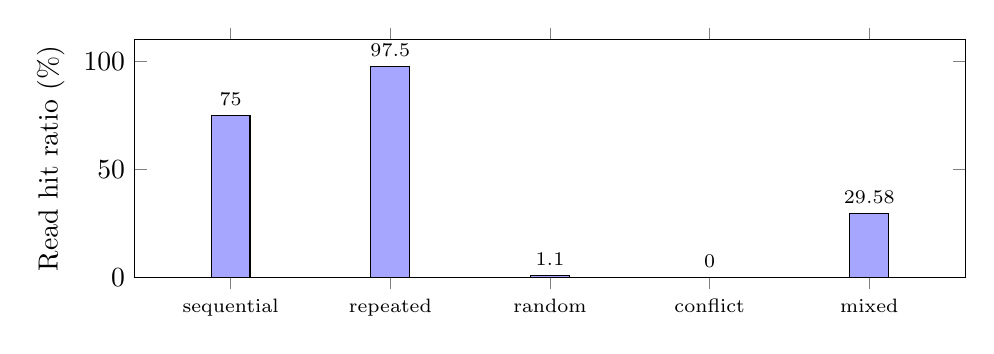
\begin{tikzpicture}
\begin{axis}[ybar, width=\columnwidth, height=4.6cm, ymin=0, ymax=110,
  ylabel={Read hit ratio (\%)}, symbolic x coords={sequential,repeated,random,conflict,mixed}, xtick=data,
  x tick label style={font=\scriptsize}, nodes near coords, bar width=14pt,
  every node near coord/.append style={font=\scriptsize}, enlarge x limits=0.15]
\addplot[fill=blue!35] coordinates {(sequential,75.00) (repeated,97.50) (random,1.10) (conflict,0.00) (mixed,29.58)};
\end{axis}
\end{tikzpicture}

\caption{Read hit ratio for each trace.}
\label{fig:hit}
\end{figure}

\begin{itemize}
\item \textbf{Sequential (75\%)}: each block holds 4 words, so the first word misses and the next three hit. This is
spatial locality: the hit ratio is $1 - 1/4$ and would rise with larger blocks.
\item \textbf{Repeated (97.5\%)}: the 512-byte array (32 blocks) fits in the 1~KB cache. Only the 32 compulsory misses
of the first pass occur, so the hit ratio is $1 - 32/1280$. This is temporal locality.
\item \textbf{Random (1.1\%)}: the cache holds only 1/64 of the 64~KB address range, so almost every access is a
capacity or compulsory miss.
\item \textbf{Conflict (0\%)}: the two addresses map to the same line and evict each other on every access, although
the rest of the cache is empty. This is the main weakness of direct mapping; a 2-way set-associative cache or a
victim cache~\cite{jouppi1990} would turn all but the first two accesses into hits.
\item \textbf{Mixed (29.6\%)}: the 2~KB region is twice the cache size and write misses do not allocate, so many
reads miss. Of the 58 writes, 20 hit and updated the cache; all 58 were written to memory.
\end{itemize}

\subsection{Effect of the miss penalty}
Fig.~\ref{fig:amat} repeats the read-only traces for memory latencies from 5 to 100 cycles. For the repeated trace
AMAT grows only from 2.18 to 4.55 cycles, because only 2.5\% of accesses pay the penalty. For the random and
conflict traces AMAT grows almost one-for-one with the latency (from about 9 to 103--104 cycles). A high hit ratio is therefore
more and more important as the gap between processor and memory speed grows.

\begin{figure}[t]
\centering
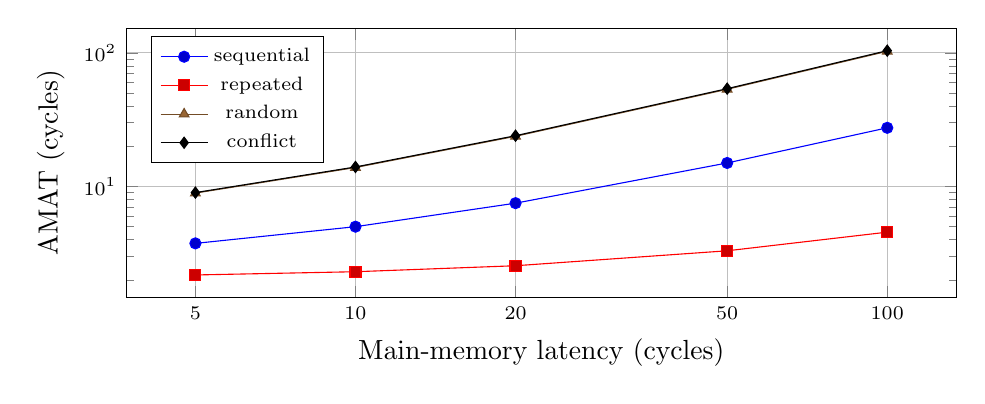
\begin{tikzpicture}
\begin{axis}[width=\columnwidth, height=5cm, xlabel={Main-memory latency (cycles)},
  ylabel={AMAT (cycles)}, xmode=log, ymode=log, log basis x=10,
  xtick={5,10,20,50,100}, xticklabels={5,10,20,50,100},
  legend pos=north west, legend style={font=\scriptsize}, grid=major,
  tick label style={font=\scriptsize}]
\addplot+[mark=*] coordinates {(5,3.750) (10,5.000) (20,7.500) (50,15.000) (100,27.500)};
\addlegendentry{sequential}
\addplot+[mark=square*] coordinates {(5,2.175) (10,2.300) (20,2.550) (50,3.300) (100,4.550)};
\addlegendentry{repeated}
\addplot+[mark=triangle*] coordinates {(5,8.923) (10,13.868) (20,23.758) (50,53.428) (100,102.878)};
\addlegendentry{random}
\addplot+[mark=diamond*] coordinates {(5,9.000) (10,14.000) (20,24.000) (50,54.000) (100,104.000)};
\addlegendentry{conflict}
\end{axis}
\end{tikzpicture}

\caption{Measured AMAT against main-memory latency (log scales). The random and conflict curves almost overlap.}
\label{fig:amat}
\end{figure}

\subsection{Synthesis}
The cache (without the main-memory model) was synthesised with Yosys for a Xilinx 7-series FPGA
(Table~\ref{tab:synth}). The 64-entry RAMs are mapped to distributed (LUT) RAM because they are read
asynchronously. The flip-flops hold the request registers, the 64 valid bits and the FSM state. Most of the 197
input and 103 output buffers come from the wide 128-bit memory bus, which would be internal in a full processor.

\begin{table}[h]
\centering
\caption{Yosys synthesis results (Xilinx 7-series)}
\label{tab:synth}
\begin{tabular}{lr}
\toprule
Resource & Count \\
\midrule
LUTs (LUT2--LUT6) & 316 \\
Flip-flops (FDRE) & 138 \\
Distributed RAM (RAM64M) & 136 \\
CARRY4 & 2 \\
I/O buffers (IBUF/OBUF) & 197 / 103 \\
\bottomrule
\end{tabular}
\end{table}

\subsection{Limitations}
The main memory is a behavioural model with a fixed latency, accesses are whole 32-bit words, and the CPU waits
for each access to finish (no pipelining). Write-through sends every store to memory; a write-back cache with dirty
bits would reduce memory traffic for programs with many stores.

% ======================================================================
\section{Individual Contributions}
Table~\ref{tab:contrib} lists the main work of each member. Each member committed their own modules to the shared
GitHub repository, and all members reviewed the integrated design and the report.

\begin{table}[h]
\centering
\caption{Individual contributions}
\label{tab:contrib}
\begin{tabular}{>{\raggedright\arraybackslash}p{2.1cm}>{\raggedright\arraybackslash}p{5.6cm}}
\toprule
Member & Contribution \\
\midrule
Asad Ali & Tag/index/offset derivation; \texttt{address\_decoder} and \texttt{tag\_comparator} modules \\
Divyansh Bhartia & Cache storage: \texttt{data\_ram}, \texttt{tag\_ram}, \texttt{valid\_ram} with reset of valid bits \\
Vikrant Yadav & \texttt{main\_memory} model and memory interface; trace generator (\texttt{gen\_traces.py}) \\
Mayank Pillai & Controller FSM (\texttt{cache\_controller}) and top-level integration (\texttt{cache\_top}) \\
Prashant Raj & Self-checking testbench, hit/miss statistics, AMAT and latency sweep, Yosys synthesis \\
\bottomrule
\end{tabular}
\end{table}

% ======================================================================
\section{Conclusion}
We designed a 1~KB direct-mapped cache with 16-byte blocks in Verilog, built from an address decoder, valid, tag and
data RAMs, a tag comparator and a four-state controller FSM. A self-checking testbench confirmed correct lookup,
refill, valid-bit handling and write-through on six traces with no data errors. The results match the theory
exactly: sequential access gives a 75\% hit ratio from spatial locality, a loop that fits in the cache gives 97.5\%
from temporal locality, and two addresses 1~KB apart give 0\% because of conflict misses. The measured AMAT equals
$2 + \text{miss rate} \times 12$ cycles for a 10-cycle memory, and the design fits in about 316 LUTs and 138
flip-flops on a Xilinx 7-series FPGA. Future work includes a 2-way set-associative version with LRU replacement to
remove the conflict misses, a write-back policy, and a study of block and cache size.

% ======================================================================
\begin{thebibliography}{9}
\bibitem{hennessy2017} J.~L. Hennessy and D.~A. Patterson, \emph{Computer Architecture: A Quantitative Approach},
6th~ed. Cambridge, MA, USA: Morgan Kaufmann, 2017.
\bibitem{patterson2020} D.~A. Patterson and J.~L. Hennessy, \emph{Computer Organization and Design RISC-V Edition:
The Hardware/Software Interface}, 2nd~ed. Cambridge, MA, USA: Morgan Kaufmann, 2020.
\bibitem{smith1982} A.~J. Smith, ``Cache memories,'' \emph{ACM Computing Surveys}, vol.~14, no.~3, pp.~473--530,
1982.
\bibitem{hill1988} M.~D. Hill, ``A case for direct-mapped caches,'' \emph{Computer}, vol.~21, no.~12, pp.~25--40,
Dec. 1988.
\bibitem{hill1989} M.~D. Hill and A.~J. Smith, ``Evaluating associativity in CPU caches,'' \emph{IEEE Trans.
Computers}, vol.~38, no.~12, pp.~1612--1630, Dec. 1989.
\bibitem{jouppi1990} N.~P. Jouppi, ``Improving direct-mapped cache performance by the addition of a small
fully-associative cache and prefetch buffers,'' in \emph{Proc. 17th Annu. Int. Symp. Computer Architecture (ISCA)},
1990, pp.~364--373.
\bibitem{denning2005} P.~J. Denning, ``The locality principle,'' \emph{Communications of the ACM}, vol.~48, no.~7,
pp.~19--24, 2005.
\bibitem{ieee1364} \emph{IEEE Standard for Verilog Hardware Description Language}, IEEE Std 1364-2005, 2006.
\bibitem{iverilog} S.~Williams, ``Icarus Verilog.'' [Online]. Available: \url{https://steveicarus.github.io/iverilog/}
\bibitem{yosys} C.~Wolf, ``Yosys Open SYnthesis Suite.'' [Online]. Available: \url{https://yosyshq.net/yosys/}
\end{thebibliography}

\end{document}
